\chapter{Požiadavky a návrh riešenia}

\label{kap:navrh_riesenia}

\section{Analýza požiadavkov}

Cieľom je vytvoriť webovú aplikáciu ktorá bude schopná vizualizovať výsledky meraní internetu v grafickej forme pomocou diagramov, 
grafov a máp. 

\subsection{Požiadavky na beh aplikácie}

Požiadavky na beh serverovej časti:
\begin{itemize}
    \item Systém musí byť schopný pracovať s PostgreSQL
    \item Systém nesmie zapisovať do databázy s meraniami
    \item Všetky časti systému musia byť schopné bežať na Linuxovom prostredí (CentOS alebo Ubuntu)
    \item Systém musí byť schopný priebežne predspracovávať namerané dáta po týždňoch, 
    aby boli vizualizácie zobrziteľné ihneď (bez dlhého čakania)
    \item Systém nesmie byť závislý od vonkajších služieb iných, ako databáza s meraniami 
    (lokalizačné servisy aj mapové servery musia bežať vrámci systému)
    \item Spracovanie dát pre jeden týždeň nesmie trvať viac ako jeden týždeň (nutné preto, aby spracovanie niekedy dobehlo)
\end{itemize}
Požiadavky na beh klientskej časti:
\begin{itemize}
    \item Aplikácia musí fungovať na všetkých moderných prehliadačoch
    \item Aplikácia musí vedieť vizualizácie zobrazovať bez pridlhého načítavania
\end{itemize}

Detaily implementácie boli ponechané na moje uváženie. Detaily rozhodovania sú popísané v kapitole \ref{kap:moznosti_implementacie}.

Serverový systém bude implementovaný na .NET 6.0. Systém bude pozostávať z niekoľkých aplikácií, z ktorých jedna bude pôsobiť ako 
server pre klientskú časť, jedna bude pôsobiť ako API pre získavanie spracovaných dát a zvyšné budú služby bežiace na pozadí, ktoré budú mať za úlohu
priebežne spracovávať namerané dáta. Predspracované dáta sa budú ukladať do PostgreSQL 15.0 databázy. Tieto služby budú spúšťané plánovačom úloh
jedenkrát týždenne. Systém bude bežať v niekoľkých kontaineroch v platforme Docker. Ako samostatný kontainer bude bežať databáza, API na prístup k 
dátam, NGINX server pre klientskú aplikáciu, každý background worker a Open Street Maps tile server. Ako údaje na lokalizáciu ip adries bude 
použitá voľná CSV databáza DB-IP lite \cite{ip_city_db}.

Klientská časť bude implementovaná pomocou systému Angular 15.0. API bude volané pomocou vstavanej knižnice httpClient. Na zobrazenie 
presnej geografickej mapy sveta budú použité Open Street Maps pomocou knižnice Leaflet a jej wrapperu pre Angular ngx-leaflet. Na zobrazenie 
mapy sveta po krajinách je použitý mierne upravený verejne voľný svg template \cite{svg_mapa}.

\section{Používateľské scenáre}
Keďže služby bežiace na pozadí nebudú mať žadneho používateľa a budú fungovať samy bez vstupu od používateľa, je potrebné navrhnúť len scenáre 
pre frontendovú aplikáciu.

\subsection{Používateľské scenáre pre frontendovú aplikáciu}
\label{scenare}
Aplikácia bude mať len jeden typ používateľa. Keďže celá webová čast je len na čítanie, nie je pootrebné obmedzovať práva pre niektorých používateľov. 
Z tohto dôvodu sme sa rozhodli vynechať autentifikáciu a aplikáciu sprístupniť bez mena a hesla.

Po spustení aplikácie bude vidieť domovskú obrazovku. Tá bude pozostávať z navigačného menu, mapy sveta s vyznačenými skupinami 
uzlov IP adries na základe ich geografickej polohy. Menu bude obsahovať dve položky, domovská obrazovka a mapa krajín. Na stránke bude prepínač týždňov, 
ktorým sa bude ovládať voľba týždňa, pre ktorý chceme, aby sa dáta zobrazili. Tiež sa na stránke bude nachádzať výberový zoznam na výber medzi prezeraním 
maximálnych, priemerných alebo minimálnych dôb odozvy. Po zmene stavu prepínačov sa zmeny v dátach prejavia okamžite pri všetkých troch selektoroch. 
V mape sa tiež bude nachádzať legenda podľa ktorej sa bude dať určiť hodnota odozvy podľa farby kruhu znázorňujúceho uzol a počet IP adries reprezentovaných 
kruhom podľa veľkosti priemeru kruhu. Pri maximálnom priblížení sa pri kruhoch zobrazia detailné informácie o údajoch nameraných v daný týždeň.

Po kliknutí na mapu krajín v menu sa zobrazí druhá stránka. Tá bude obshovať rovnaké menu ako domovská stránka. V hlavnej časti bude mapa krajín sveta. 
Krajiny budú zafarbené podľa doby odozvy pre danú krajinu. Nad mapou sa bude nachádzať prepínač týždňov a rovnaké výberové zoznamy ako na domovskej stránke. 
V mape sa tiež bude nachádzať legenda na priradenie doby odozvy k farbe.

\subsection{Návrh rozhrania na komunikáciu so serverovou časťou}
Rozhranie by malo fungovať podľa architektonického štýlu \uv{REST}. To určuje niekoľko pravidiel, medzi nimi napríklad oddelenosť backendu od frontendu, 
komunikáciu pomocou protokolu HTTP alebo nezávislosť dopytov jeden od druhého \cite{rest}. Rozhranie by malo obsahovať tieto metódy:
\begin{itemize}
    \item \verb|GET /CountryPingInfo/ForWeek/{week}| (parameter week - ISO 8601 reprezentácia týždňa) - Metóda, ktorá vráti dáta o dobe odozvy pre všetky odmerané krajiny pre daný týždeň. 
    \begin{lstlisting}[language={TypeScript},caption={Vzorový výstup z endpointu},label=alg:get_country_ping_info_example]
        [
            {
                "id": 0,
                "week": "2022-W05",
                "ipAddressesCount": 0,
                "averagePingRtT": 0,
                "maximumPingRtT": 0,
                "minimumPingRtT": 0,
                "countryCode": "SK"
            }
        ]
    \end{lstlisting}
    \item \verb|GET /CountryPingInfo/ColoredMap/{week}| (parameter week - ISO 8601 reprezentácia týždňa) - Metóda ktorá vráti SVG obrázok s mapou sveta s krajinami zafarbenými podľa doby odozvy pre daný týždeň. 
    \begin{lstlisting}[language={XML},caption={Vzorový výstup z endpointu},label=alg:get_country_ping_info_map_example]
        <?xml version="1.0" encoding="utf-8"?>
        <svg width="2000" height="857" fill="#ECECEC" stroke="black" stroke-width=".2"...
            <path id="AF" class=" AF" d="M1383,261.6l1.5,1.8 -2.9,.8 -2.4,1.1 -5.9,.8 -5.3,1.3 ...
            <path class="Angola AO " d="M1121.2,572 1121.8,574 1121.1,577.1 1122,580.1 1121.1, ...
            <path class="Angola AO " d="M1055.3,539 1053.8,534.2 1056.1,531.4 1057.8,530.3 ...
            ...
    \end{lstlisting}
    \item \verb|GET /CountryPingInfo/LastProcessedDate| - Metóda, ktorá vráti posledný týždeň, pre ktorý sú spracované dáta o dobe odozvy pre krajiny.
    \begin{lstlisting}[language={TypeScript},caption={Vzorový výstup z endpointu},label=alg:last_date_example]
        {
            "response": "string"
        }
    \end{lstlisting}
    \item \verb|GET /MapPoints/ForWeek/{week}| (parameter week - ISO 8601 reprezentácia týždňa) - Metóda, ktorá vráti dáta o dobe odozvy pre všetky odmerané body na mape podľa polohy pre daný týždeň. 
    \begin{lstlisting}[language={TypeScript},caption={Vzorový výstup z endpointu},label=alg:get_map_points_info_example]
        [
            {
                "id": 0,
                "week": "2022-W05",
                "ipAddressesCount": 0,
                "averagePingRtT": 0,
                "maximumPingRtT": 0,
                "minimumPingRtT": 0,
                "latitude": 0,
                "longitude": 0
            }
        ]
    \end{lstlisting}
    \item \verb|GET /MapPoints/LastProcessedDate| - Metóda, ktorá vráti posledný týždeň, pre ktorý sú spracované dáta o dobe odozvy pre geograficcké lokality.
    Vzorový výstup je zhodný s ukážkou \ref{alg:last_date_example}.
    \item \verb|GET /MapPoints/MapPointsMapLegend| - Metóda, ktorá vráti svg obrázok legendy vykreslený podľa zadaných parametrov. Parametre by mali obsahovať 
    definíciu piatich dvojíc veľkosť-počet, ktoré budú znázorňovať veľkosť kruhu a počet adries znázorňujúci túto veľkosť.
    \begin{lstlisting}[language={XML},caption={Vzorový výstup z endpointu},label=alg:legend_example]
        <?xml version="1.0" encoding="utf-8"?>
        <svg viewBox="0 0 500 300" width="500" height="300" xmlns="http://www.w3.org/2000/svg">
            <rect x="1.622" y="5.63" ...
            <ellipse ...
            ...
            <text ...
            ...
            <rect ...
            <ellipse ...
            ...
            <text ...
        </svg>
    \end{lstlisting}
\end{itemize}

\subsection{Návrh lokálnej databázy}
Databázový pokytovateľ bude PostgreSQL vo verzií 15. Databáza bude bežať vo vyhradenom kontajneri. Databáza bude pozostávať z troch tabuliek. 
    
Tabuľka \lstinline{ipadresses} - Pomocná tabuľka pri napĺňaní zvyšných tabuliek. Bude obsahovať zoznam známych IP adries s informáciou 
o ich geografickej lokalite. Bude naplnená ako prvá, skôr ako zvyšné 2 tabuľky. Bude pozostávať z nasledovných stĺpcov:
\begin{itemize}
    \item id - celé číslo - primárny kľúč
    \item ipvalue - IPV4 adresa vo formáte cidr - konkrétna hodnota IP adresy na ktorú sa riadok vzťahuje
    \item countrycode - reťazec o dĺžke maximálne 2 znakov - ISO 3166-1 Alpha 2 kód krajiny, v ktorej sa nachádza IP adresa
    \item city - reťazec o dĺžke maximálne 80 znakov - názov mesta, v ktorom sa nachádza IP adresami
    \item latitude - reálne číslo - zemepisná šírka IP adresy
    \item longitude - reálne číslo - zemepisná dĺžka IP adresy
\end{itemize}

Tabuľka \lstinline{countrypinginfo} bude obsahovať 
informácie o nameraných dobách odozvy zoskupených podľa krajín. Bude pozostávať z nasledovných stĺpcov:
\begin{itemize}
    \item id - celé číslo - primárny kľúč
    \item countrycode - reťazec o dĺžke maximálne 2 znakov - ISO 3166-1 Alpha 2 kód krajiny, o ktorej riadok hovorí
    \item week - reťazec o dĺžke maximálne 8 znakov - ISO 8601 reprezentácia týždňa, pre ktorý je riadok platný
    \item averagepingrtt - celé číslo - zaokrúhlena priemerná hodnota odozvy pre danú krajinu v danom týždni
    \item maximumpingrtt - celé číslo - maximálna doba odozvy pre danú krajinu v danom týždni
    \item minimumpingrtt - celé číslo - minimálna doba odozvy pre danú krajinu v danom týždni
\end{itemize}

Tabuľka \lstinline{mapiprepresentation} bude obsahovať informácie o nameraných dobách 
odozvy zoskupených podľa geografickej lokality. Bude pozostávať z nasledovných stĺpcov:
\begin{itemize}
    \item id - celé číslo - primárny kľúč
    \item latitude - reálne číslo - priemerná zemepisná šírka všetkých IP adries zoskupených v danom riadku v danom týždni
    \item longitude - reálne číslo - priemerná zemepisná dĺžka všetkých IP adries zoskupených v danom riadku v danom týždni
    \item week - reťazec o dĺžke maximálne 8 znakov - ISO 8601 reprezentácia týždňa, pre ktorý je riadok platný
    \item averagepingrtt - celé číslo - zaokrúhlena priemerná hodnota odozvy pre danú krajinu v danom týždni
    \item maximumpingrtt - celé číslo - maximálna doba odozvy pre danú krajinu v danom týždni
    \item minimumpingrtt - celé číslo - minimálna doba odozvy pre danú krajinu v danom týždni
\end{itemize}

Tabuľky medzi sebou nebudú nijako prepojené, pretože by to neprinieslo žiadnu výhodu vzhľadom na charakter 
meraných dát. Entitno-relačný diagram je viditeľný na obrázku \ref{obr:entitn_diagram}.

Databáza bude obsahovať aj indexy. Indexy sú štruktúra, ktorá umnožňuje zrýchliť vyhľadávanie v databáze na úkor spomalenia zápisu \cite{db_index}. 
Čas nás v násom systéme zaujíma hlavne z hľadiska používania webovej aplikácie. Tá z databázy výlučne číta. Zápis budeme naopak robiť len raz do týždňa 
a na čase pri ňom príliš nezáleží (jediné obmedzenie je, že spracovanie týždňa musí trvať menej ako týždeň, čo je veľmi štedrý čas). Vzhľadom na to je 
takáto optimalizácia v našom systéme veľmi vítaná. Keďže systém môže bežať dlhý čas, spracované údaje sa môžu stať priveľké a vyhľadávanie v nich bez 
indexácie by bolo veľmi pomalé. Zároveň jednoznačné indexy vedia zaručiť väčšiu konzistentnosť dát, keďže vedia zaručiť, že kombinácie niektorých údajov 
sa môžu v tabuľke vyskytnúť maximálne raz \cite{index_strategy}.

Okrem primárneho kľúča v každej tabuľke ich bude 5. Pôjde o index zaručujúci jedinečnosť IP adresy v tabuľke 
\lstinline{ipadresses}, index zaručujúci jedinečnosť kombinácie zemepisnej šírky, dĺžky a týždňa v tabuľke \lstinline{mapiprepresentation}, index na 
optimalizáciu vyhľadávania podľa týždňa v tabuľke \lstinline{mapiprepresentation}, index zaručujúci jedinečnosť kombinácie krajiny a týždňa v tabuľke 
\lstinline{countrypinginfo} a index na optimalizáciu rýchlosti vyhľadávania podľa týždňa v tabuľke \lstinline{countrypinginfo}.

\begin{figure}
    \centerline{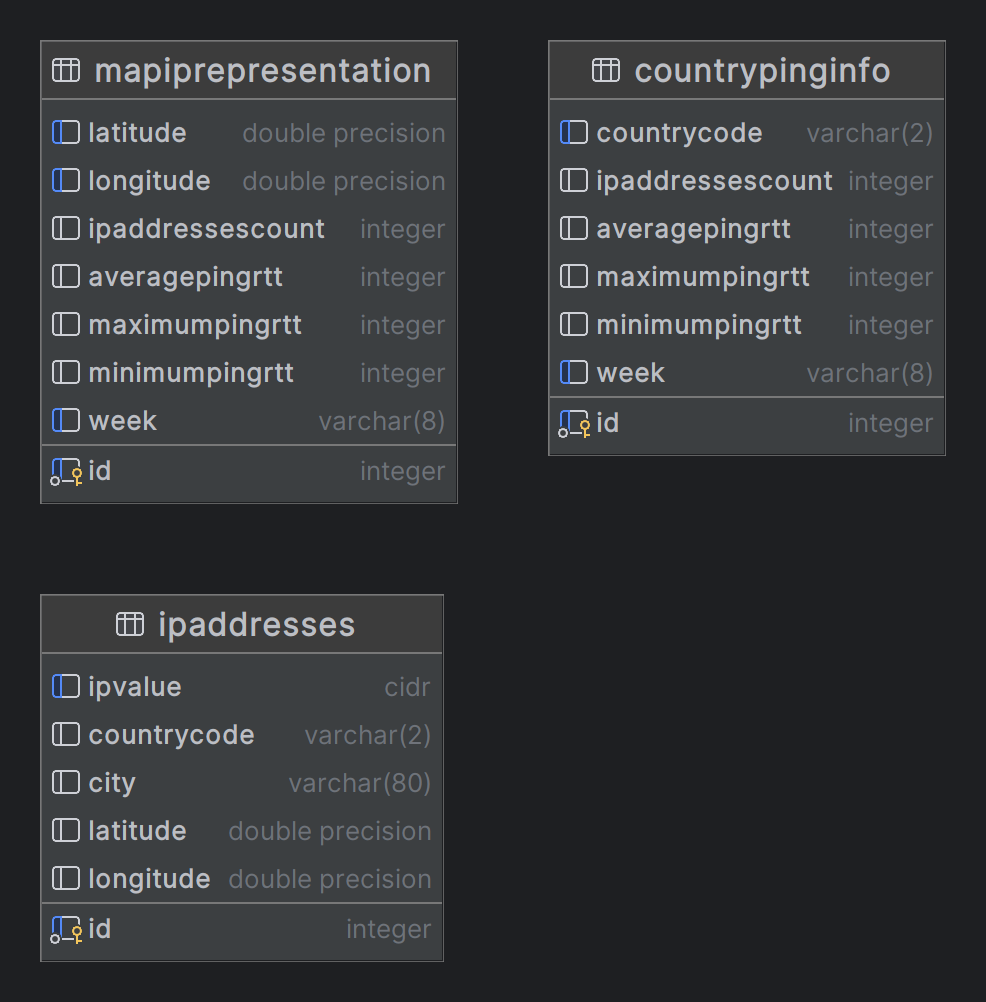
\includegraphics[width=0.8\textwidth]{images/ipinfoviewerprocesseddb}}
    %popis obrazku
    \caption[Entitno-relačný digram k lokálnej databáze]{Entitno-relačný digram k lokálnej databáze. 
    Na obrázku je vidno, že tabuľky nie sú nijako previazané}.
    %id obrazku, pomocou ktoreho sa budeme na obrazok odvolavat
    \label{obr:entitn_diagram}
\end{figure}